\section{Data Analysis}
In the given data, there are some numerical and categorical features:
\begin{itemize}
    \item \emph{Numerical}: \texttt{temp}, \texttt{dew}, \texttt{humidity}, \texttt{precip}, \texttt{snow}, \texttt{snowdepth}, \texttt{windspeed}, \texttt{cloudcover} and \texttt{visibility}.
    \item \emph{Categorical}: \texttt{hour\_of\_day}, \texttt{day\_of\_week}, \texttt{month}, \texttt{holiday}, \texttt{weekday}, \texttt{summertime}, and \texttt{increase\_stock}
\end{itemize}

\begin{figure}[htbp]
    \centering
    \begin{subfigure}{0.3\textwidth}
        \centering
        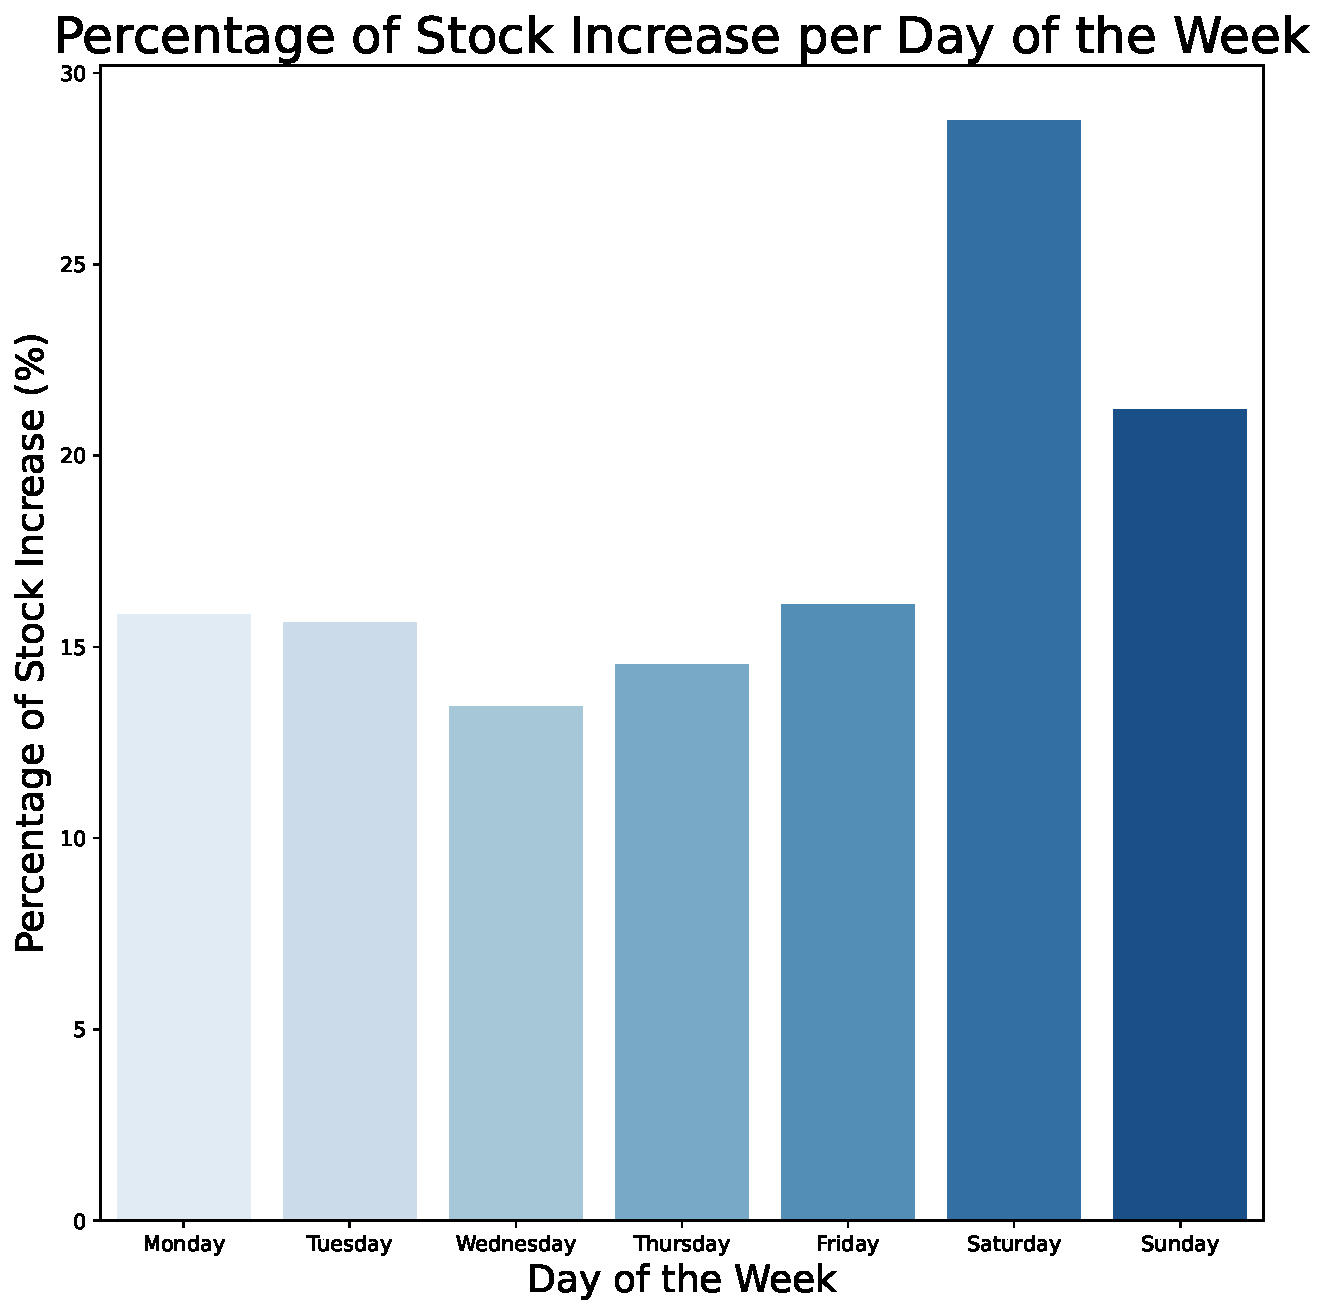
\includegraphics[width=\textwidth]{demand_day.pdf}
        \caption{Demand per day of week.}
        \label{fig:demand day}
    \end{subfigure}
    \hfill
    \begin{subfigure}{0.3\textwidth}
        \centering
        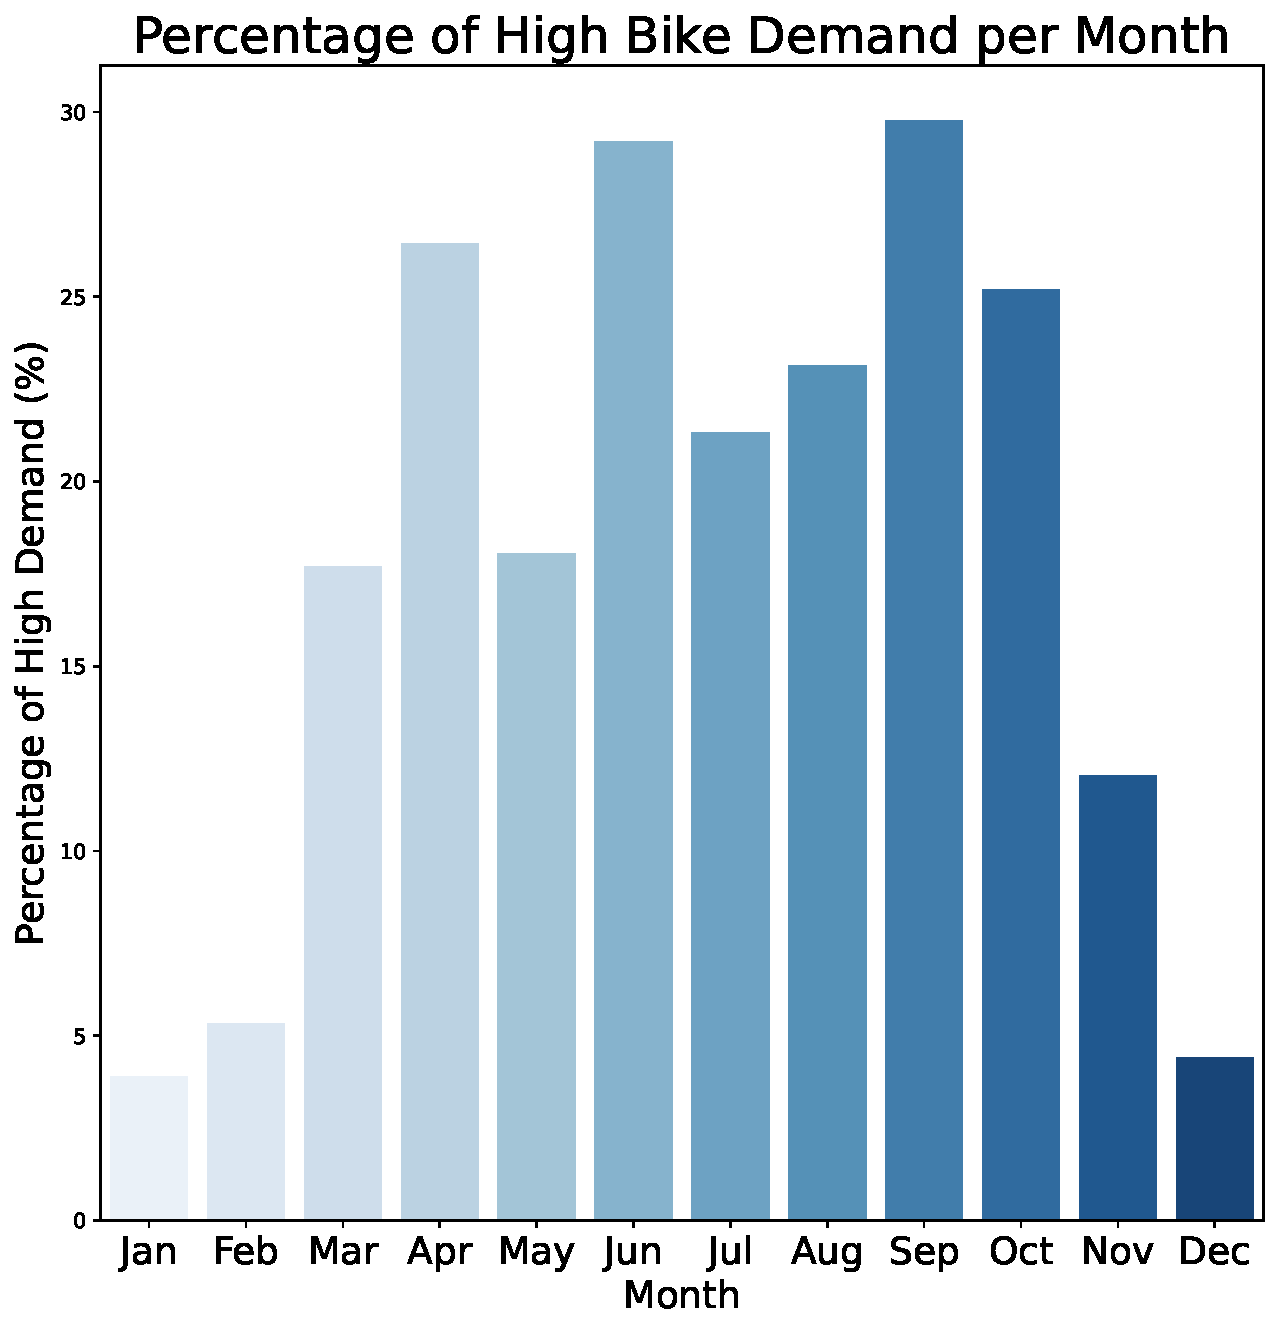
\includegraphics[width=\textwidth]{demand_month.pdf}
        \caption{Demand per month.}
        \label{fig:demand month}
    \end{subfigure}
    \hfill
    \begin{subfigure}{0.3\textwidth}
        \centering
        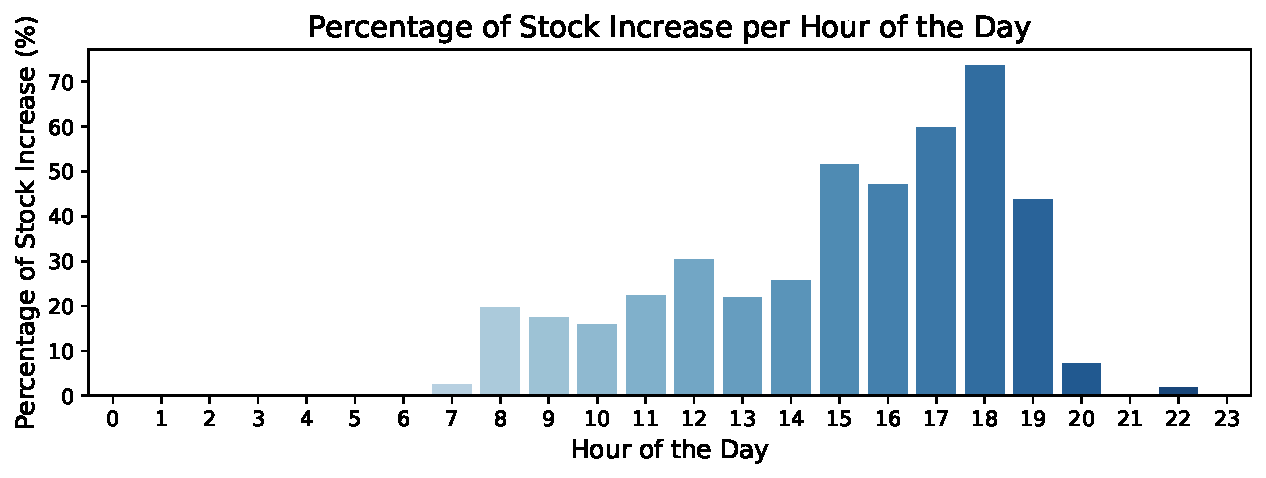
\includegraphics[width=\textwidth]{demand_hour.pdf}
        \caption{Demand per hour of day.}
        \label{fig:demand hour}
    \end{subfigure}
    \caption{Bike demand vs. day of week and month.}
    \label{fig:demand day month}
\end{figure}

\begin{figure}[htbp]
    \centering
    
    \caption{Bike demand vs. tempreature LÄGG IN FLER HÄR TYP.}
    \label{fig:demand time of day}
\end{figure}
% Gör en bra figure här med alla typ idk, även holiday.

There are some trends seen in the data when it comes to time and weather. From figure \ref{fig:demand day month}, one can see a periodic relationship for the months, where there is a higher demand during the warmer months, loosely following a trigonometric curve. Over the week, the demand is rather stable, with a peak on the weekend, especially saturdays. Looking at the weather; if there is rain or if there is snow on the ground, there is close to always low demand. Cloudcover did not make a big impact, which is also intuitive, as a cloudy day does not make biking more difficult. Dew point also does not have a clear trend, while humidity however has a clear trend downwards as the humidity increases.

The overall trend is that about one eigth of observations correspond to a high bike demand. During the night, or in bad weather, the demand is (intuitively) low. But during rush hour (fig. \ref{fig:demand time of day}), the demand is very high, and should probably be increased in order to minimize excessive CO$_2$ emissions.